Hemos dicho que la metodología de diseño que vamos a usar es Kanban, pero a mi personalmente me gusta siempre dar una serie de diagramas y de ideas procedentes del clásico desarrollo en cascada. Ya que las metodologías ágiles tienen unos entregables determinados y en ninguno de ellos aparecen los que yo voy a exponer a continuación, pero me parecen de una gran importancia y además expresan conceptos a nivel de arquitectura que a mi parecer deben de tener toda construcción de software. 

\subsubsection*{Elicitación de requisitos}

\textcolor{red}{Puede ser interesante meter una pequeña sección describiendo los requisitos funcionales y no funcionales de la aplicación, pero puede que sea introducir mucho la metodología en cascada}

\subsubsection*{Diagrama de clases de alto nivel}

\textcolor{red}{introducir un diagrama de clases aunque sea bastante simple? Puede estar interesante para mostrar los diferentes objetos que vamos a tener en representación a las tablas de la base de datos, pensar en ello}

\subsubsection*{Diagrama de casos de uso}

\textcolor{red}{lo equivalente al diagrama de casos de uso van a ser las diferntes US con el backlog, no se hasta que punto merece la pena ponerlo}

\subsubsection*{Diagrama de paquetes de alto nivel}

Uno de los diagramas que refleja muy bien la arquitectura que va a tener el sistema es el diagrama de paquetes, en el se suelen representar los diferentes paquetes y clases principales de las que se va a componer la aplicación. Podemos observar de un vistazo los principales patrones utilizados, así como las principales interacciones entre las diferentes partes que componen el sistema. 

El diagrama de paquetes, con los principales patrones que más se adecúan a la solución es el mostrado en la \textbf{Figura \ref{fig:diagramaPaquetes}}.

En esta arquitectura a alto nivel se puede apreciar el uso del modelo MVC, donde habrá clases que representen a la vista y accedan al modelo usando un controlador general de aplicación. Luego dicho controlador de aplicación es el que se encargará de interactuar con el resto de elementos y de proveer la información. 

Una de las partes más importantes de esta aplicación es el acceso a los datos, ya que vamos a estar interactuando de manera permanente contra una base de datos. Dichas peticiones tienen que ser eficientes y realizarse en el menor tiempo posible y de una manera sencilla. El patrón por el que he optado ha sido un patrón basado en objetos, es decir nosotros vamos a crear un ORM (Object Request Manager), que se va a encargar de atender las peticiones de información y va a devolver las filas de la base de datos en forma de objetos. 

Nuestra aplicación verá la base de datos como grandes listas de objetos. Cada de una base de datos será representada por un objeto diferente, con tantos atributos como columnas tenga dicha tabla. Cuando la aplicación necesite consultar una de esas filas, lo que hace nuestro ORM es devolver una lista con todas las filas de la base de datos en forma de lista de objetos. Entonces la aplicación se encarga de realizar la búsqueda dentro de esa lista. 

\begin{figure}[H]
    \centering
    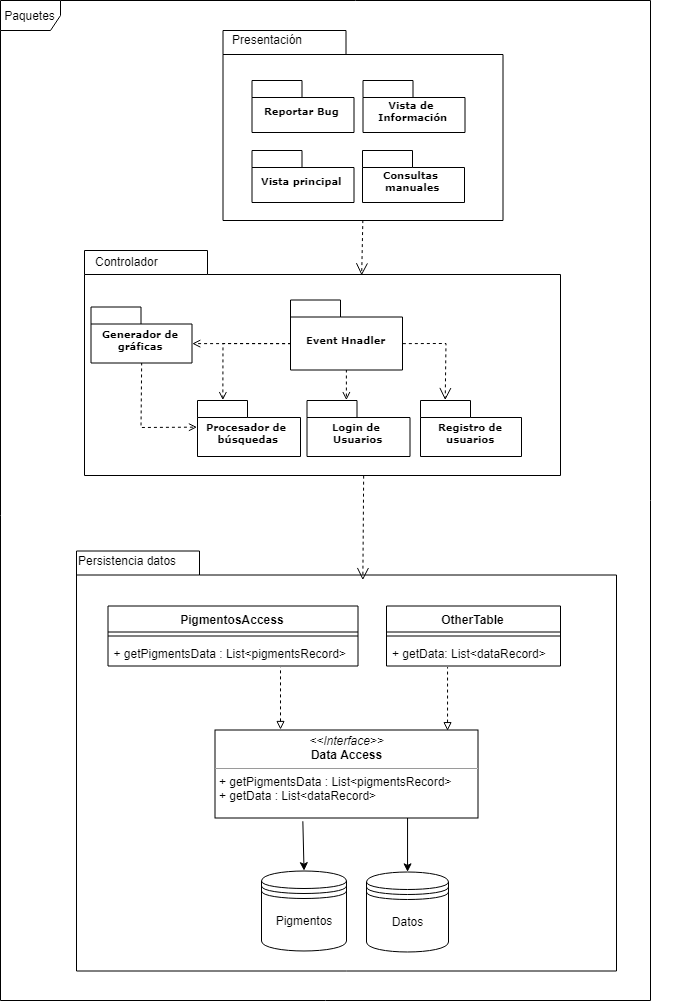
\includegraphics[scale=0.6]{imagenes/diseno/arquitecturaAltoNivel.png}
    \caption{Diagrama de Paquetes a alto nivel}
    \label{fig:diagramaPaquetes}
\end{figure}

\subsubsection*{Diagramas de secuencia de alto nivel}

En esta sección vamos a ilustrar como sería la interacción básica de los componentes de alto nivel de la aplicación. No buscamos una fuente detalla de los datos sino simplemente una aproximación a la solución que hemos planteado para que se entienda lo que hemos desarrollado en la aplicación, pero sin entrar a detalles de bajo nivel que pueden ofuscar la presentación. 

En este caso vamos a especificar un diagrama de secuencia para el supuesto de que el usuario quiere observar las propiedades químicas de un pigmento determinado. Esta secuencia de actividades la podemos ver reflejada a modo de ejemplo en el diagrama de la \textbf{Figura \ref{fig:diagramaSecuenciaVerPigmento}} 

\textcolor{red}{Hay que poner un OPT en el diagrama de secuencias, si tiene la información simplemente tiene que ir al objeto a buscarla, pero si no tiene que hacer otra consulta mediante el ORM para extraer la información de las tablas de la base de datos.}

\textcolor{red}{Igual hay que mirar de introducir algún diagrama de secuencia más, pero en principio este caso representa la funcioanldiad casi completa y básica de la aplicaicón}

\begin{figure}[H]
    \centering
    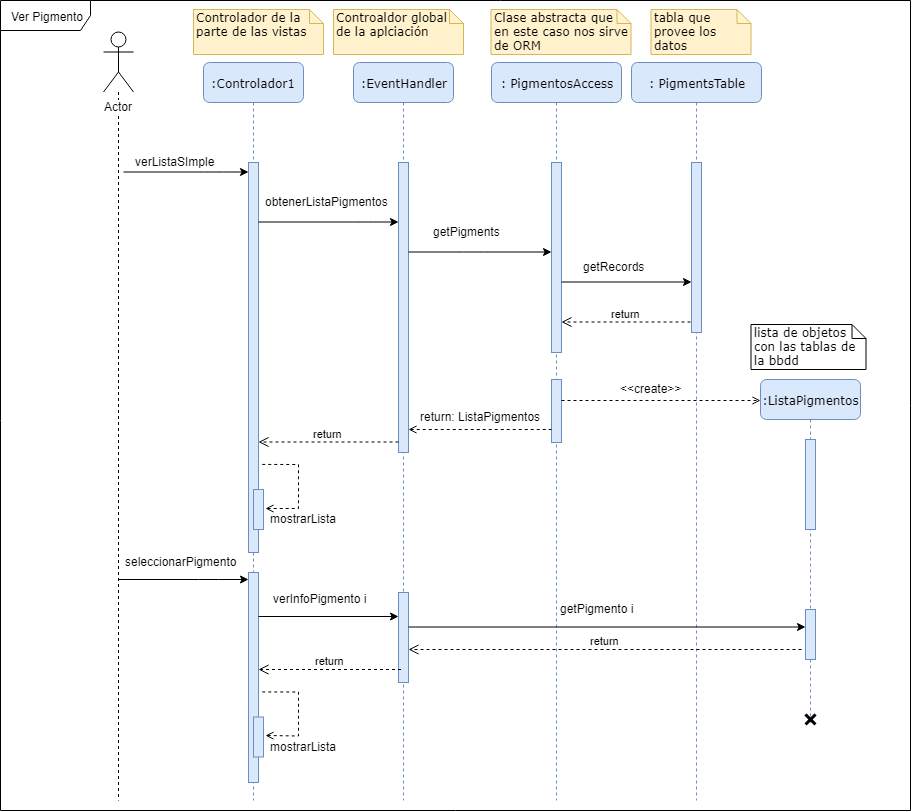
\includegraphics[scale=0.5]{imagenes/diseno/verInfoPigmentoSecuencia.png}
    \caption{Diagrama de secuencia de alto nivel para ver la información de un pigmento}
    \label{fig:diagramaSecuenciaVerPigmento}
\end{figure}

En este diagrama a de secuencias para uno de los casos más básicos, podemos observar como el actor interactúa con la aplicación y toca en el botón de ver todos los pigmentos, esta acción desencadena que el controlador del MVC se ponga en contacto con el controlador principal de la aplicación. Dicho controlador interactúa con el ORM que hemos dicho antes. Este ORM hace la consulta necesaria MySQL en la base de datos y le devuelve al controlador de aplicación una lista con todos los objetos representando las filas de la tabla que se haya consultado, en este caso la general de los pigmentos. El controlador de aplicación devuelve la información al controlador de la vista y presenta la información de una manera adecuada para el usuario. 

Ahora el usuario selecciona un pigmento en concreto, para ello el controlador de las vistas se pone en contacto con el controlador de la aplicación, el cuál no necesita interactuar con la base de datos porque ya tienes los datos disponibles. Buscamos el pigmento en cuestión, devolvemos la información al controlador de aplicación y este devuelve la información al controlador de las vistas. Hecho esto la el usuario tiene a su disposición la información que quería. 

Una vez que hemos presentado los principales diagramas e ideas en el formato tradicional, vamos a seguir con nuestra metodología inicial que es Kanban. 

